\documentclass[12pt, twoside]{article}
\usepackage[letterpaper, margin=1in, headsep=0.2in]{geometry}
\setlength{\headheight}{0.6in}
%\usepackage[english]{babel}
\usepackage[utf8]{inputenc}
\usepackage{microtype}
\usepackage{amsmath}
\usepackage{amssymb}
%\usepackage{amsfonts}
\usepackage{siunitx} %units in math. eg 20\milli\meter
\usepackage{yhmath} % for arcs, overparenth command
\usepackage{tikz} %graphics
\usetikzlibrary{quotes, angles}
\usepackage{graphicx} %consider setting \graphicspath{{images/}}
\usepackage{parskip} %no paragraph indent
\usepackage{enumitem}
\usepackage{multicol}
\usepackage{venndiagram}

\usepackage{fancyhdr}
\pagestyle{fancy}
\fancyhf{}
\renewcommand{\headrulewidth}{0pt} % disable the underline of the header
\raggedbottom
\hfuzz=2mm %suppresses overfull box warnings

\usepackage{hyperref}

\fancyhead[LE]{\thepage}
\fancyhead[RO]{\thepage \\ Name: \hspace{4cm} \,\\}
\fancyhead[LO]{BECA / Dr. Huson / Geometry\\*  Unit 11: Circle angles, sectors, arcs \\* 2 March 2023}

\begin{document}

\subsubsection*{11.4 Classwork: Inscribed angles}
\begin{enumerate}

\item Given the circle with center $P$ with central angle $\angle APB$ and inscribed angle $\angle AQB$. Using a protractor, measure each angle.
\begin{multicols}{2}
  \raggedcolumns
  \begin{enumerate}
    \item $m\angle APB=$ \vspace{0.7cm}
    \item $m\angle AQB=$ \vspace{0.7cm}
    \item What do you think is the ratio of the central angle to the inscribed angle?
  \end{enumerate}
    \begin{tikzpicture}[scale=.8]
      \draw (0,0) circle[radius=5];
      \draw [thick]
      (-20:5) node[right] {$B$}--
      (0,0) node[below] {$P$}--
      (80:5) node[above left] {$A$};
      \draw [thick] (-20:5)--(210:5) node[below left] {$Q$}--(80:5);
      %\draw (60:5) node[right]{$130^\circ$};
    \end{tikzpicture}
\end{multicols}

\item Given circle $O$ with chords $\overline{AD}$ and $\overline{BE}$ intersecting at $C$, as shown in the diagram, which is drawn to scale. Use a protractor to measure each angle and a ruler for (e).
    \begin{multicols}{2}
    \raggedcolumns
    \begin{enumerate}[itemsep=1cm]
      \item Find the $m\angle A$.
      \item Find the $m\angle B$.
      \item Find the $m\angle D$.
      \item Find the $m\angle E$.
      \item Given that $BE=8$ \\[0.25cm] 
      Find $BC$.
      \item Find $EC$.
    \end{enumerate}
    \begin{tikzpicture}[scale=1]
      \draw (0,0) circle[radius=4];
      \draw [thick]
      (-60:4) node[right] {$E$}--
      (120:4) node[above left] {$B$}--
      (200:4) node[left] {$A$}--
      (50:4) node[above right] {$D$}--cycle;
      \draw (140:0.9) node[below] {$C$};
    \end{tikzpicture}
    \end{multicols}
  \vspace{2cm}

\item The diagram below shows $\triangle ABC \sim \triangle ADE$, with $\overline{AEB}$, $\overline{ADC}$. $AB=12$, $AD=6$. Estimate $BC$, assuming that the diagram below is drawn to scale.
\begin{multicols}{2}
  Write the actual lengths of 
  \begin{enumerate}
    \item $AB=$ \vspace{0.7cm}
    \item $AD=$ \vspace{0.7cm}
    \item $BC=$  \vspace{0.7cm}
    \item Find the scale factor, $k$ \vspace{1.2cm}
    \item Calculate $BC=$
  \end{enumerate}
    \begin{tikzpicture}[scale=1.5]
      \draw [thick]
      (0,0) node[above right] {$A$}--
      (230:6) node[below left] {$B$}--
      (260:4.75) node[below right] {$C$}--cycle;
      \draw [thick]
      (230:2.375) node[above left] {$E$}--
      (260:3) node[right] {$D$}--cycle;
    \end{tikzpicture}
  \end{multicols}\vspace{1.5cm}


\begin{multicols}{2}
\item Given circle $P$ with $m \wideparen{AB}=120^\circ$.
  \raggedcolumns
  \begin{enumerate}
    \item Write down the $m\angle APB$. \vspace{1cm}
    \item Find the $m\angle AQB$. \vspace{2cm}
  \end{enumerate}
    \begin{tikzpicture}[scale=.4]
      \draw (0,0) circle[radius=5];
      \fill (0,0) circle[radius=0.15];
      \draw [thick]
      (-20:5) node[right] {$B$}--
      (0,0) node[below] {$P$}--
      (100:5) node[above left] {$A$};
      \draw [thick] (-20:5)--(210:5) node[below left] {$Q$}--(100:5);
      \draw (60:5.2) node[right]{$120^\circ$};
    \end{tikzpicture}
\end{multicols}
  
\item Given circle $O$ with chords $\overline{AD}$ and $\overline{BE}$ intersecting at $C$, as shown in the diagram. Given $m \wideparen{AB}=45^\circ$, $m \wideparen{BD}=110^\circ$, and $m \wideparen{DE}=65^\circ$.
  \begin{multicols}{2}
  \raggedcolumns
  \begin{enumerate}[itemsep=1cm]
    \item Find the $m\angle BAD$.
    \item Find $m \wideparen{AE}$
    \item Find the $m\angle ABE$.
    \item Find the $m\angle ACB$.
  \end{enumerate}
  \begin{tikzpicture}[scale=.5]
    \draw (0,0) circle[radius=5];
    \draw [thick]
    (-10:5) node[right] {$E$}--
    (150:5) node[left] {$B$}--
    (200:5) node[left] {$A$}--
    (60:5) node[above right] {$D$}--cycle;
    \draw (140:1.4) node[below] {$C$};
    \draw (30:5) node[right] {$65^\circ$};
    \draw (100:5) node[above] {$110^\circ$};
    \draw (175:5) node[left] {$45^\circ$};
  \end{tikzpicture}
  \end{multicols}
  
\newpage
\item Given circle $O$ with chords $\overline{AD}$ and $\overline{BE}$ intersecting at $C$, as shown in the diagram. Given $m \wideparen{AB}=70^\circ$, $m \wideparen{BD}=80^\circ$, and $m \wideparen{DE}=110^\circ$.
  \begin{multicols}{2}
    \raggedcolumns
    \begin{enumerate}[itemsep=1.5cm]
      \item Find the $m\angle BED$.
      \item Find the $m\angle ACB$.
      \item Given $AC=4$ and $BC=3$, find $AB$.
      \item Given $CE=6$, find $CD$.
    \end{enumerate}
    \begin{tikzpicture}[scale=.6]
      \draw (0,0) circle[radius=5];
      \draw [thick]
      (-60:5) node[right] {$E$}--
      (130:5) node[left] {$B$}--
      (200:5) node[left] {$A$}--
      (50:5) node[above right] {$D$}--cycle;
      \draw (160:1.3) node[below] {$C$};
      \draw (120:3.5) node[below] {$3$};
      \draw (190:3) node[below] {$4$};
      \draw (280:2.0) node[below] {$6$};
      \draw (0:5) node[right] {$110^\circ$};
      \draw (100:5) node[above] {$80^\circ$};
      \draw (165:5) node[left] {$70^\circ$};
    \end{tikzpicture}
  \end{multicols} \vspace{2cm}
  
\item The secants $\overline{ABC}$ and $\overline{ADE}$ intersect the circle $O$, as shown in the diagram. \\Given $m \wideparen{BD}=28^\circ$ and $m \wideparen{CE}=136^\circ$.
\begin{enumerate}
    \begin{multicols}{2}
      \item Find the $m\angle CDE$.
      \item Find the $m\angle BCD$.
    \end{multicols}  \vspace{1.5cm}
  \item Find the $m\angle A$. \vspace{0.5cm}
\end{enumerate}
  \begin{center}
  \begin{tikzpicture}[scale=.6]
    \draw (0,0) circle[radius=5];
    \draw [thick]
    (3,-4) node[below right] {$E$}--
    (-5,0) node[below left] {$D$}--
    (-9,2) node[left] {$A$}--
    (55:5) node[above right] {$C$}--
    (-5,0);
    \draw (138:5) node[left] {$B$};
    \draw (0:5) node[right] {$136^\circ$};
    \draw (160:5) node[left] {$28^\circ$};
  \end{tikzpicture}
\end{center}

\item Given the circle with center $P$ with central angle $\angle APB$ and inscribed angle $\angle AQB$. The intercepted arc has a measure $m \wideparen{AB}=78^\circ$.
  \begin{multicols}{2}
    \raggedcolumns
    \begin{enumerate}
      \item Find $m\angle APB=$ \vspace{0.7cm}
      \item Find $m\angle AQB=$ \vspace{0.7cm}\\
      Circle True or False:
      \begin{enumerate}[itemsep=0.3cm]
        \item T \, F \, $\overline{AP}$ is a radius
        \item T \, F \, $\overline{AQ}$ is a chord
        \item T \, F \, $\angle APB$ is a central angle
      \end{enumerate}
    \end{enumerate}
      \begin{tikzpicture}[rotate=100, scale=.5]
        \draw (0,0) circle[radius=5];
        \fill (0,0) circle[radius=0.1];
        \draw [thick]
        (-10:5) node[above] {$B$}--
        (0,0) node[below] {$P$}--
        (70:5) node[left] {$A$};
        \draw [thick] (-10:5)--(200:5) node[below right] {$Q$}--(70:5);
        \draw (30:5.2) node[left]{$78^\circ$};
      \end{tikzpicture}
  \end{multicols} \vspace{0.25cm}

\end{enumerate}
\end{document}